\section{Apache ServiceMix}
\label{sec:servicemix}  

In this diploma thesis we extend a multi-tenant aware version of Apache ServiceMix 4.3.0, referred to it in this document as ServiceMix. Essl evaluates different available \ac{ESB} solutions in the market, and as output of his work provides a selection decision for extending ServiceMix in order to support multi-tenancy \cite{Essl2011}. As mentioned in Section \ref{sec:multitenancy}, a multi-tenant \ac{ESB} solution in a \ac{PaaS} environment must support tenant-aware communication, and tenant-aware administration and management. The support is provided by Muhler and Gomez in their corresponding works in \cite{Muhler2012}, \cite{gomez2012}, leading to a multi-tenant ServiceMix prototype supporting different communication protocols. We will refer to it as ServiceMix-mt.

As a main difference with previous versions' architectures, ServiceMix is an integration container based on the \ac{OSGi} Framework implementation Apache Karaf  \cite{Karaf2011}. It provides a light environment in which components and applications can be deployed in a loose coupled way. Apache Karaf provides an extensible management command line console where management of the components lifecycle, such us \ac{OSGi} bundles, \ac{JBI} components or \ac{SA}s, can be done in a user friendly way (see Figure \ref{fig:servicemix}). Furthermore, a hot deployment directory is shipped with the \ac{ESB} package where users can deploy \ac{OSGi} bundles, \ac{JBI} components wrapped in \ac{SA}'s, etc. just by copying the file into it. The undeployment is done automatically when the user deletes the file from the \term{deploy} directory. 

The main advantage in the ServiceMix 4.3.0 it is its full compliance with the \ac{JBI} specification. Its \ac{JBI} container has as its main component the \ac{NMR} (See Figure \ref{fig:servicemix}). In the \ac{JBI} container users are provided with \ac{JBI} deployment support and management. The communication between the \ac{JBI} and \ac{OSGi} container, e.g. from one \ac{OSGi} service to a \ac{JBI} Binding Component can be achieved through the \ac{NMR} using its API wrapped as an already deployed \ac{OSGi} bundle. This fact eases the integration process of components between different ServiceMix's versions, and take advantage of it in this diploma thesis. Furthermore, \ac{JBI} components or endpoint configurations packed as \ac{SE} or \ac{SA} and deployed in ServiceMix are internally packed into \ac{OSGi} bundles. 

ServiceMix is shipped with different \ac{JBI} components already deployed as \ac{OSGi} bundles in its \ac{OSGi} container. In this thesis we will concentrate on the following ones: HTTP and Apache Camel. Apache Camel is a powerful open source integration framework based on \ac{EAI} \cite{Camel2011}. Furthermore, it provides a widespread list of components which support different communication protocols.  The user can configure logical endpoints between \ac{BC}s and different routing paths between them by deploying their configuration wrapped in a \ac{SA} in the \term{deploy} directory. Different Maven plugins can make the configuration of a \ac{JBI} or \ac{SE} as simple as possible by providing different built archetypes which generates the \ac{SU} files and directories where the developer can configure the component \cite{MAVEN}. Apache Camel provides a set of maven archetypes which already contain the structure for developing custom camel components.

\begin{figure}[htb]
	\centering
		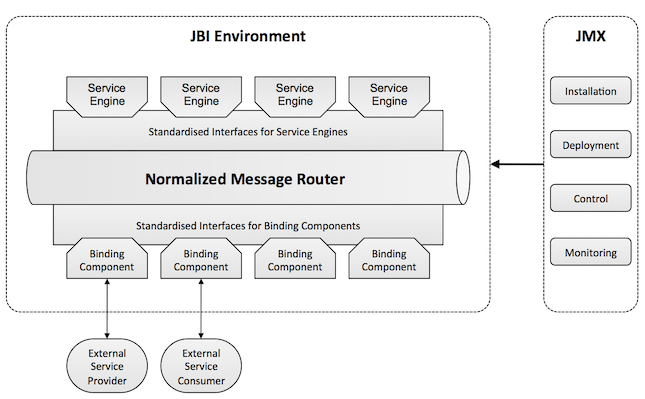
\includegraphics[clip, scale=0.4]{./gfx/servicemix.png}
	\caption[Architecture of Apache ServiceMix]{Architecture of Apache ServiceMix \cite{ASM} }
	\label{fig:servicemix}
\end{figure}

The \ac{NMR} routes the messages between the endpoints created by the \ac{JBI} components (see Figure \ref{fig:servicemix}). This endpoints are divided in two types: consumers and providers. A consumer endpoint is exposed as a service while a provider endpoint consumes an external service. When a message arrives to a consumer endpoint of a \ac{JBI} Binding Component, it is transformed into a \ac{NMF}. The \ac{NMF} is the protocol neutral format which is routed in a \ac{JBI} environment and described in Section \ref{sec:jbi}. 

The ServiceMix-mt prototype we extend in this diploma thesis already provides multi-tenant support for different communication protocols: HTTP, JMS, and E-mail. However, the data retrieval and storage in an application's architecture relies on one specific layer: Data Access Layer, and its main used communication protocols for data transfer are in most of the cases vendor specific. Communication with \ac{SQL} databases, such as MySQL, Oracle, and PostgreSQL are managed by its vendor-specific native driver, which implements the communication protocol with the database server in the \ac{DBMS}. Such protocols are not supported in the multi-tenant prototype ServiceMix-mt, and must be taken into account in the extension of the prototype in this diploma thesis. On the other hand, communication with \ac{NoSQL} databases can be also considered vendor-specific, because most of the Cloud storage providers facilitate its own API to the users to manipulate data in their data containers, but almost all of them provide either REST or \ac{SOAP} over \ac{HTTP} interfaces. This fact permits us to reuse and extend the multi-tenant HTTP \ac{BC} in ServiceMix-mt. The components we create or extend in this diploma thesis are identified by CDASMix (Cloud Data Access Support in ServiceMix-mt).

\FloatBarrier